% rxmk: engine=pdftex
% rxmk: scheme=latex

\documentclass[aspectratio=169]{beamer}

% \usepackage{tgschola} % doesn't work with the unicode engines??
\usepackage{fontspec}
\setmainfont{TeX Gyre Schola}
\setsansfont{Inter}
\usepackage{unicode-math}
\setmathfont{TeX Gyre Schola Math}

\usetheme{Singapore}
\usefonttheme{serif}

\setbeamerfont*{frametitle}{size=\LARGE, series=\scshape, parent=structure}
\setbeamerfont*{framesubtitle}{size=\large, series=\upshape\itshape, parent=structure}

\title{\scshape Translating Information Into Action}
\subtitle{\upshape SDG 3: Good Health and Well-being}
\author{Andre Poghosyan, Joanna Tang, Runxi Yu}
\date{July 31, 2025}

\setlength{\parskip}{1ex}

\begin{document}
\maketitle

\begin{frame}{Research Question}
	Previous public health campaigns often failed to improve actual hygiene behavior, despite improving knowledge.

	Can behavioral changes happen without changing what people explicitly know?

	\Large Can embedding hygiene edutainment into mobile entertainment change real handwashing behavior?

	\normalsize

	\bigskip

	\url{https://www.povertyactionlab.org/sites/default/files/research-paper/WP4378_Translating-Information-Into-Action-in-Bangladesh_Hussam-et-al_Feb2023.pdf}
\end{frame}

\begin{frame}{Subjects}
	333 households, over 23 villages, Gaibandha District, Bangladesh

	Each household has at least 1 child of primary school age;\\
	access to latrine, female head of household

	\bigskip

	No differential attrition found, but 85\% follow-up rates overall
\end{frame}

\begin{frame}{Treatment}
	\begin{columns}
	\column{0.5\textwidth}
	50\% allocated to treatment group
	\begin{itemize}
		\item Handsoap dispenser with time-stamped sensors
		\item Call-disabled smartphone with pre-loaded SD cards with
			popular dramas/cartoons, with hygiene edutainment
			(30\,s to 7\,min) embedded
		\item New SD cards delivered monthly
		\item Data is also collected about watching patterns
	\end{itemize}

	\column{0.5\textwidth}

	50\% non-treatment group
	\begin{itemize}
		\item Handsoap dispenser with time-stamped sensors
	\end{itemize}

	\bigskip\bigskip
	
	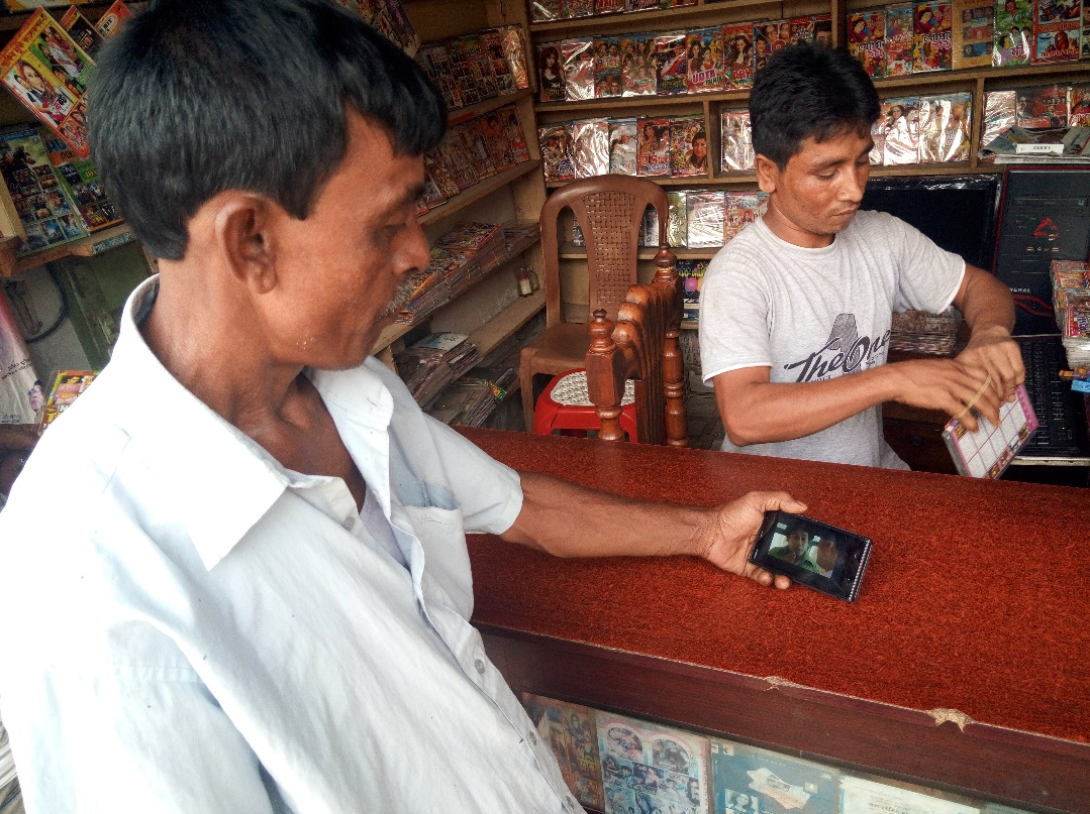
\includegraphics[scale=0.09]{img-014.png}
	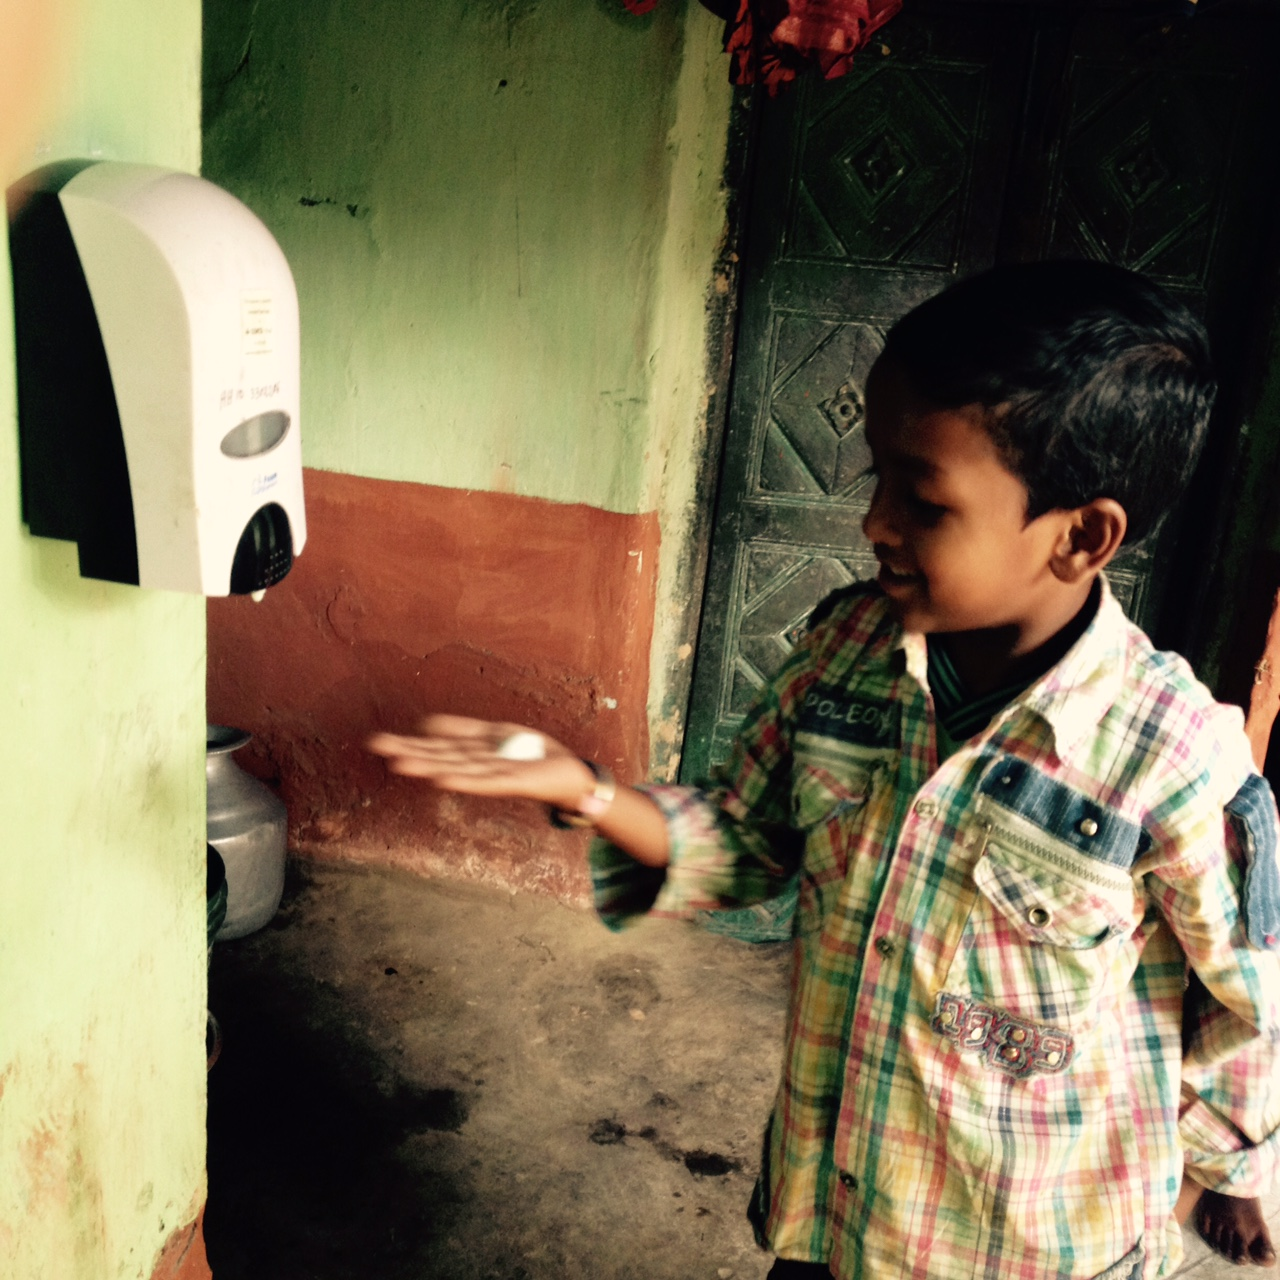
\includegraphics[scale=0.07]{img-020.png}
	\end{columns}
\end{frame}

\begin{frame}{Estimated Effects}{Engagement with Phone Entertainment}
	Treatment caused...
	\begin{itemize}
		\item Phone entertainment use to increase by 73\,pp, $p < 0.0001$
		\item Adult daily minutes watching phone to increase by 33.65\,min, $p < 0.0001$
		\item Adult watches children's cartoons to increase by 0.27\,pp, $p < 0.0001$
		\item Child phone entertainment use to increase by 0.38\,pp, $p < 0.0001$
		\item Children who use the phone daily to increase by 0.64\,pp, $p < 0.0001$
		\item Child daily minutes watching phone to increase by 17.19\,min, $p < 0.0001$
		\item Children who watch cartoons to increase by 22\,pp, $p \approx 0.0002$
	\end{itemize}

	$p$-values are estimated from the $t$-statistic, with $df \approx 280$.
\end{frame}

\begin{frame}{Estimated Effects}{Handwashing}
	\begin{columns}
	\column{0.4\textwidth}
	Treatment caused...
	\begin{itemize}
		\item No statistically significant difference in whether the dispenser is used at all on a given day, $p \approx 0.2$
		\item 22\% more times of usage per day, $p \approx 0.000$
	\end{itemize}
	Both groups are more excited to use it when they just received it.
	\column{0.58\textwidth}
	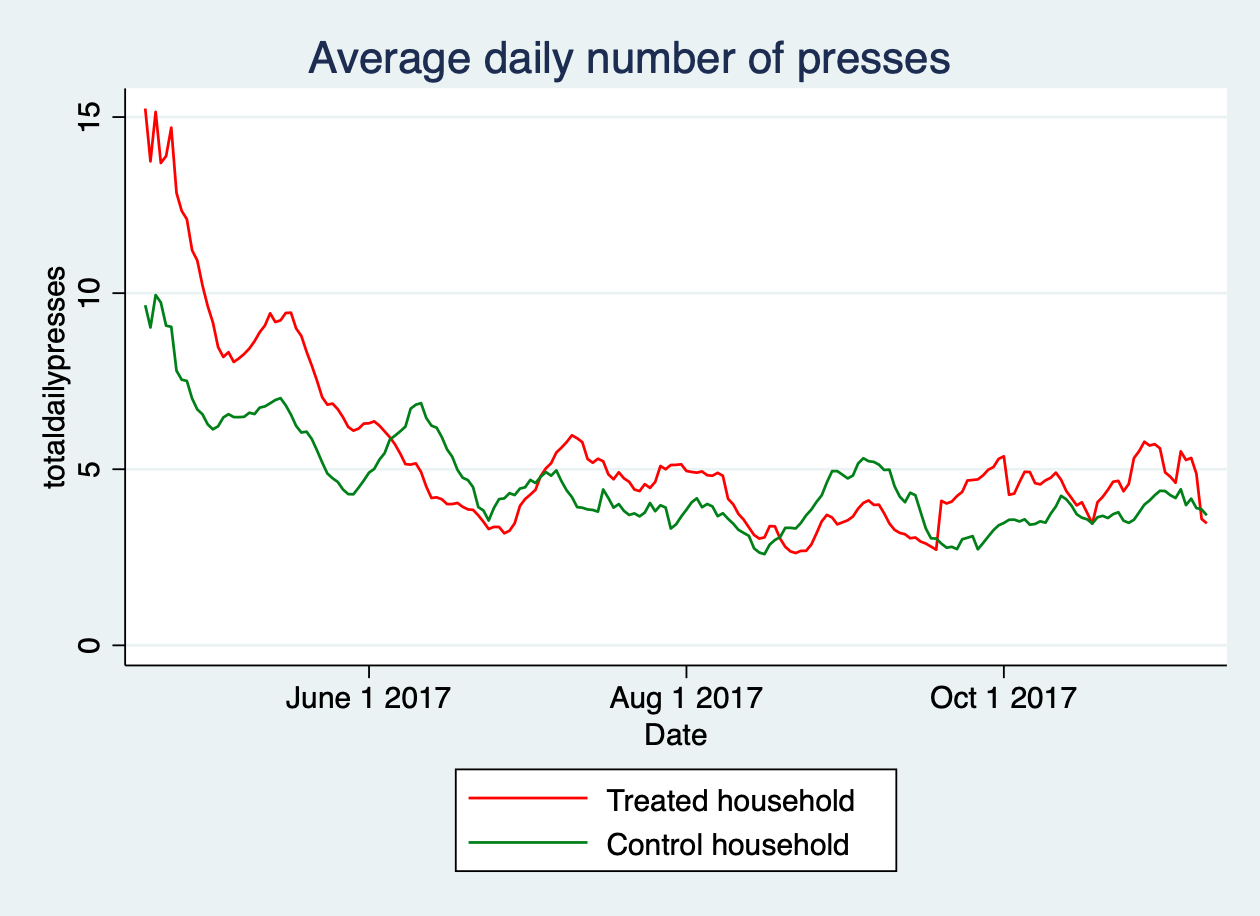
\includegraphics[width=\linewidth]{img-000.png}
	\end{columns}
\end{frame}

\begin{frame}{Wait, Why?}{Did Edutainment Improve Conscious Hygiene Knowledge?}
	When asked about what prevents colds, the ``absolute knowledge index''
	(ASI) measures whether the respondent mentions the edutainment-taught
	content, and the ``relative knowledge index'' (RSI) measures how
	prominently the content is ranked.

	ASI is improved 1.5\%, RSI improved 0.4\%, but both have $p > 0.05$.

	So no, edutainment did not consciously improve hygiene knowledge.
\end{frame}

\begin{frame}{When Do They Use the Dispenser?}{Findings from Machine Learning}
	Treated households were tracked minute-by-minute on:
	\begin{itemize}
		\item When they watched entertainment or edutainment
		\item When they used the soap dispenser
	\end{itemize}

	The best predictors of handwashing are:
	\begin{itemize}
		\item Watching edutainment in the past 3--4 weeks
		\item Watching \emph{any} entertainment in the past 30 minutes
	\end{itemize}

	So habits were formed through repeated exposure, then reinforced by watching media.
\end{frame}


\begin{frame}{Potential Confounds I}{Time Away from Peers}
	\textbf{Hypothesis:} Children watched more media, spent less time with peers, reduced illness transmission.

	Unlikely, as 17 more minutes per day is small relative to 4+ hours of school, etc.
\end{frame}

\begin{frame}{Potential Confounds II}{Phone Entertainment as a Bribe to Wash hands}
	\textbf{Hypothesis:} Parents say ``wash hands to get screen time'', which only works in families that have devices for entertainment, which all treated groups but only some untreated groups have.

	Unlikely, as:

	Households that already used phones for entertainment \emph{before} the
	experiment sitll saw large treatment effects.

	ML shows cumulative exposure to edutainment predicts hand-washing
	behavior, not just immediate access to entertainment
\end{frame}

\begin{frame}{Potential Confounds III}{Experimenter Demand Effects}
	\textbf{Hypothesis:} Treated participants behaved or responded differently to please enumerators.

	\begin{itemize}
		\item \textit{Behavioral bias:}\\``Participants used the dispenser more to signal gratitude.''

			Unlikely, as both received dispensers, and behavior changes are temporally linked to media exposure rather than surveyor visits.

		\item \textit{Health reporting bias:}\\``Treated households underreported illness to appear healthier.''

			Unlikely, as it follows seasonal expectations, and increase salience would lead to more reporting not less.
	\end{itemize}
\end{frame}

\begin{frame}{Health Outcomes}{Did Edutainment Improve Children's Health?}
	Treatment caused...
	\begin{itemize}
		\item 54\% fewer reports of loose stool (diarrhea), $p \approx 0.036$
		\item 29\% fewer symptoms of acute respiratory infection, $p \approx 0.016$
	\end{itemize}


	Effects are strongest during seasonal peaks:
	\begin{itemize}
		\item Loose stool spikes during monsoon (June–October)
		\item ARI symptoms peak in early winter
	\end{itemize}


	No statistically significant changes in:
	\begin{itemize}
		\item Water treatment
		\item Latrine use
		\item Other hygiene practices
	\end{itemize}

	So handwashing is the likely channel behind these health improvements.
\end{frame}

\begin{frame}{Health Outcomes}{Plots and diagrams}
	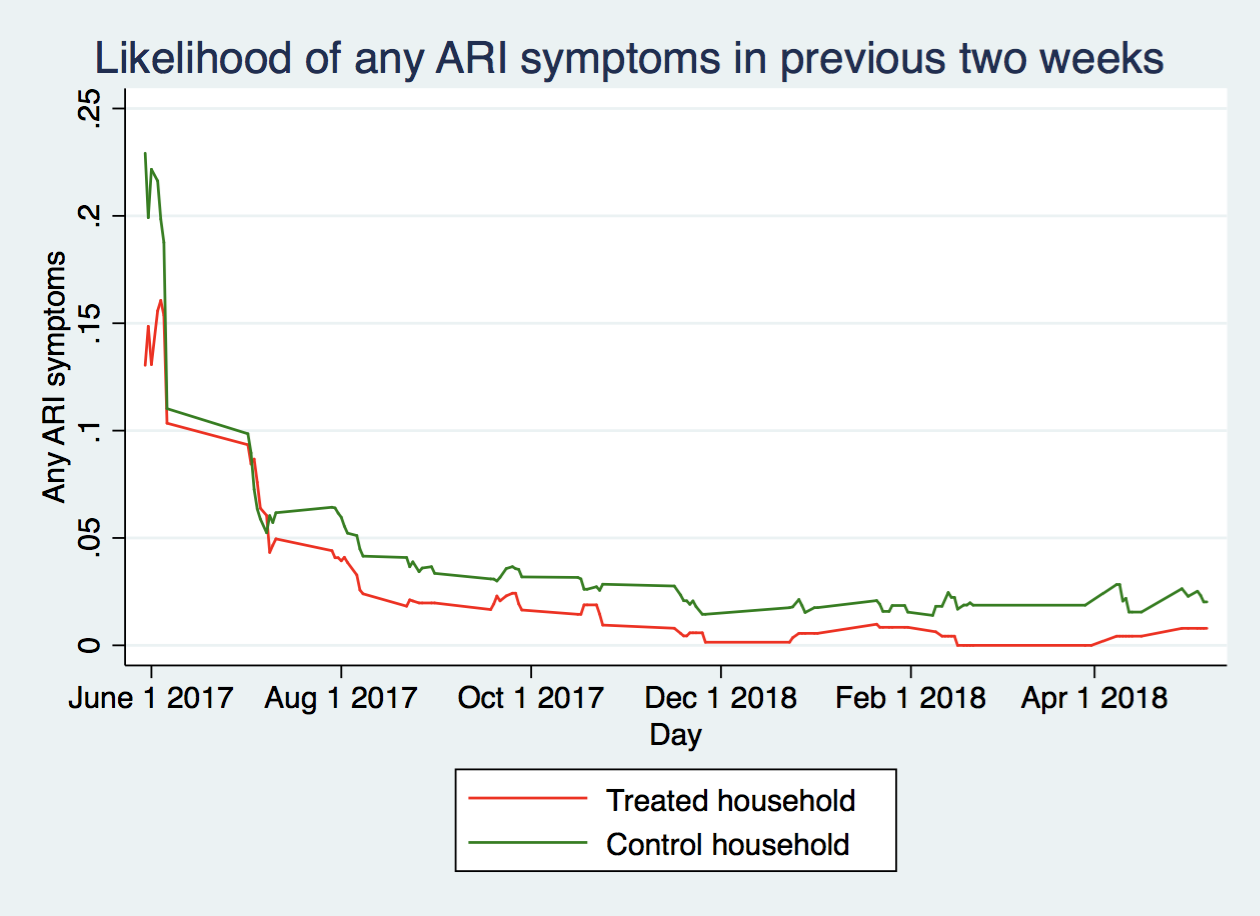
\includegraphics[width=0.48\textwidth]{img-004.png}
	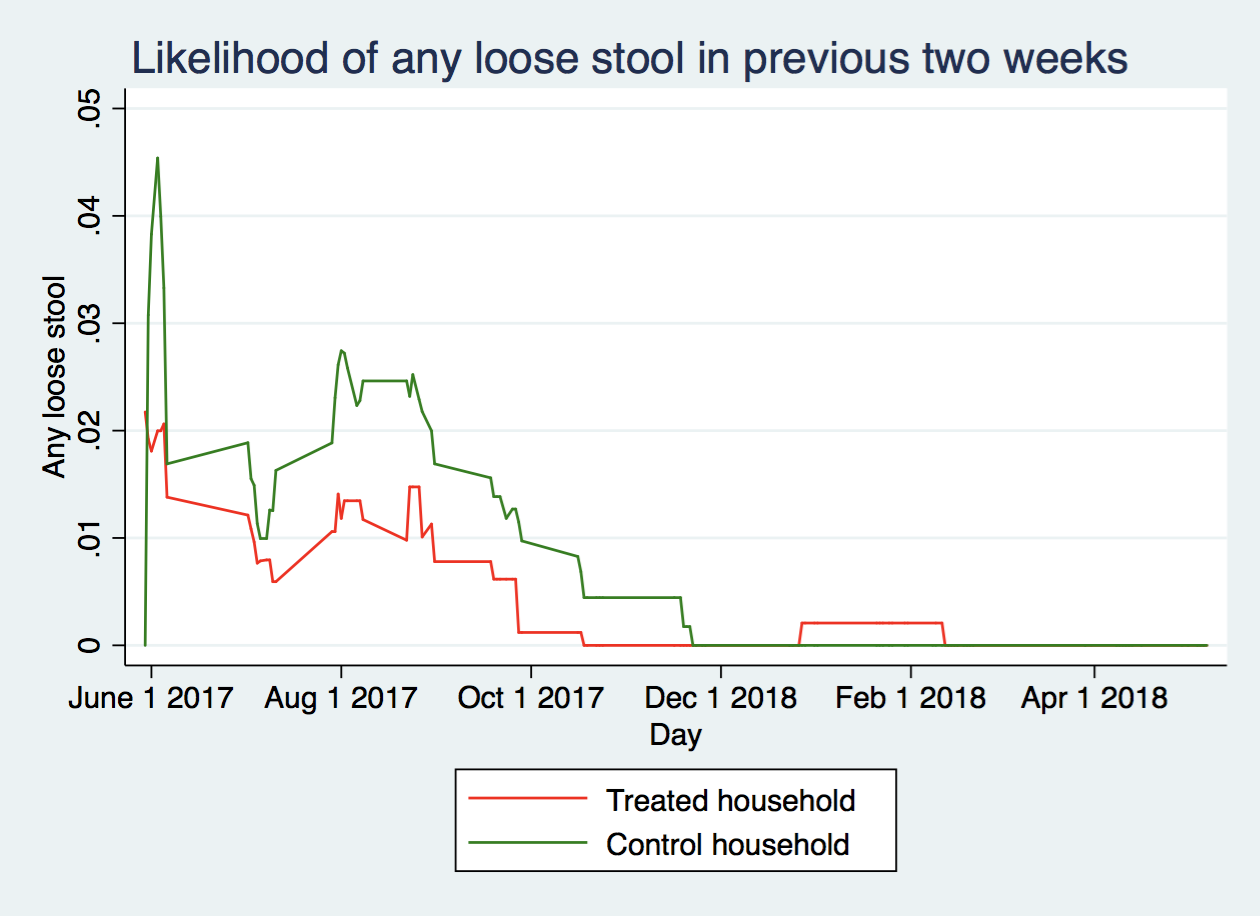
\includegraphics[width=0.48\textwidth]{img-006.png}
\end{frame}

\begin{frame}{Dispenser Alone}{How Much Did the Dispenser Help Without Edutainment?}
	A “pure control” group (no dispenser, no edutainment) was added midway for comparison.

	Compared to pure controls, households with just the dispenser (no edutainment) had:
	\begin{itemize}
		\item 68\% fewer reports of loose stool, $p \approx 0.015$
		\item 52\% fewer ARI symptoms, $p \approx 0.029$
	\end{itemize}

	Effects appear quickly and follow seasonal trends.

	So the dispenser alone has large health benefits, although edutainment still adds more.
\end{frame}

\begin{frame}{Dispenser Alone}{Plots and diagrams}
	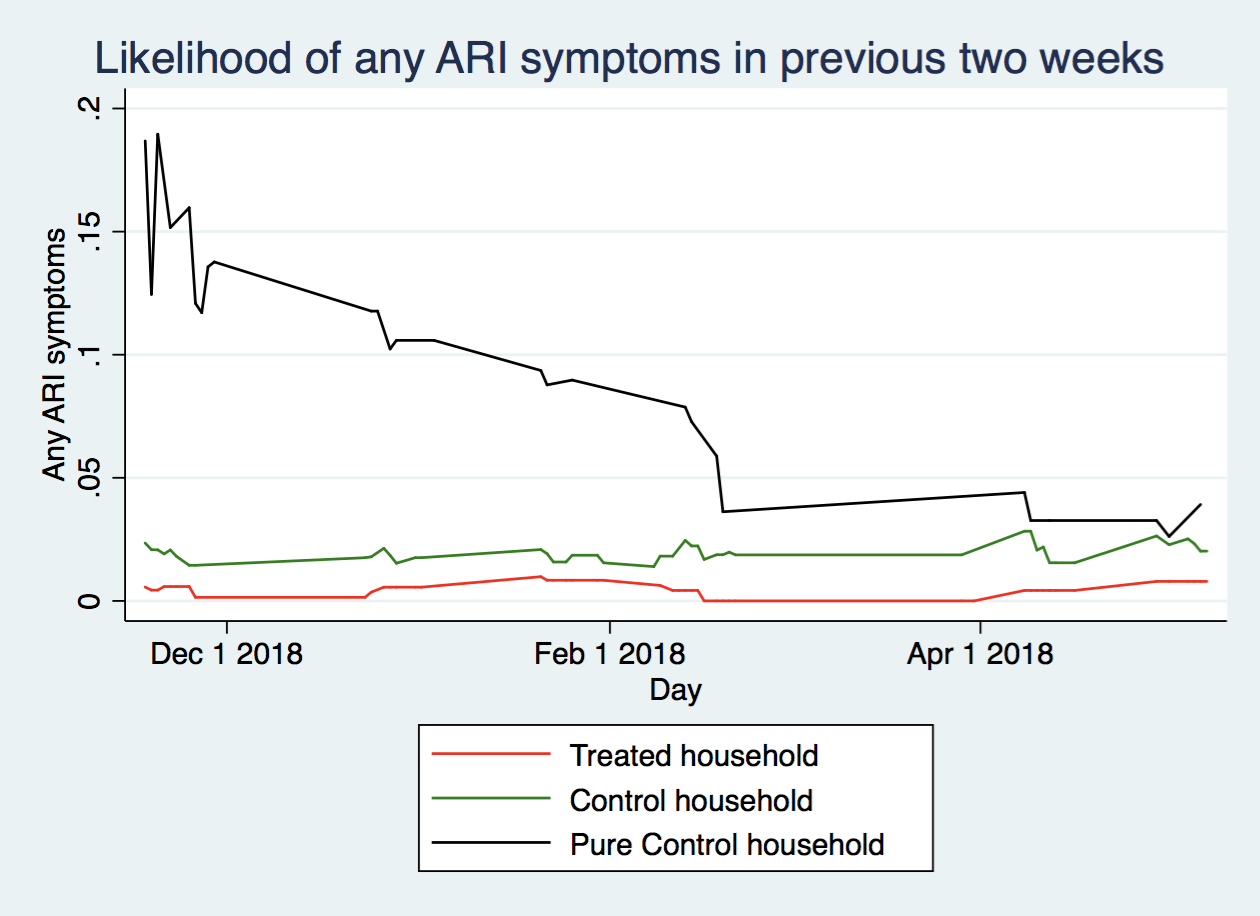
\includegraphics[width=0.48\textwidth]{img-008.png}
	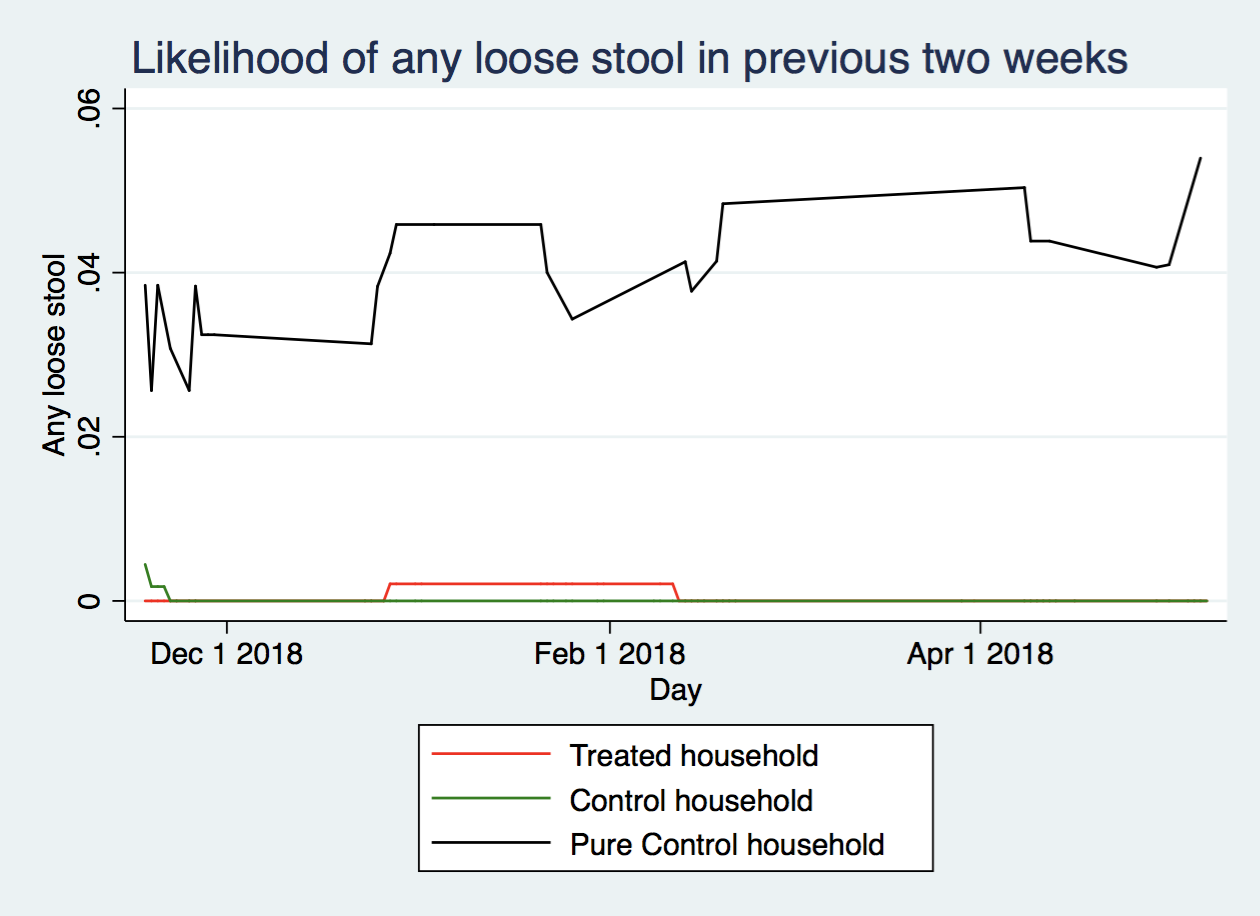
\includegraphics[width=0.48\textwidth]{img-010.png}
\end{frame}

\begin{frame}{Normative Implications}
	Repeated exposure and habit cues may matter be more important than facts in changing public health habits

	Shows that increased knowledge does not need to be the main focus of interventions as treated households washed their hands more and saw better health outcomes despite their hygiene knowledge typically remaining the same 

	Policymakers may want to focus less on lectures or info sheets and more on small reminders in daily life

	Behavior can change without changing what people believe
\end{frame}

\begin{frame}{Policy Implications}
	Embedding public health content in popular media is cheap and scalable

	Works even in low-resource settings with limited internet or literacy

	Public health agencies could deliver hygiene, vaccine, or nutrition messages through media such as movies and shows

	When trying to promote a certain type of behavior, messages should focus on frequency and simplicity over technical content 

	Phones with preloaded content could be used in areas with poor network coverage
\end{frame}

\begin{frame}
	\Huge
	\centering

	\vfill

	Thank you!

	\vfill

	\normalsize
	\flushleft


	\color{gray}Statistical significance and $p$-values are integrated through the
	presentation of results rather than listed separately.
\end{frame}


\end{document}
